\documentclass[aspectratio=169,xcolor=table]{beamer}
%aspcetratio >> 1610 169 149 54 43 32
%The themes:
%\usetheme[style=classic]{mharvellous}
%\usetheme[style=dark]{mharvellous}
\usetheme[style=classic]{mharvellous}
%\usetheme[style=default]{mharvellous}
%*--------------------------------------------------
%\usepackage{helvet}
%*--------------------------------------------------
\usepackage{bibunits}  
%\setbeamertemplate{bibliography item}{[\theenumiv]}
\setbeamertemplate{bibliography item}{\insertbiblabel}
\defaultbibliography{bibliography}
%\defaultbibliographystyle{IEEEtran}
%\defaultbibliographystyle{amsalpha}
\defaultbibliographystyle{abntex2-alf}
%\bibliography{bibliography}
%\usepackage[backend=biber,style=alphabetic,citestyle=authoryear]{biblatex}
% \addbibresource{bibliography.bib}
%\usepackage{natbib}
\usepackage{bibentry}
%*--------------------------------------------------
\usepackage{lipsum}
\usepackage{epigraph}
\usepackage{graphicx}
\usepackage{multirow}
%\usepackage{enumitem}
\usepackage{array}
%\usepackage{multimedia}
\usepackage{media9}
%\usepackage{pdfpc-movie}
\usepackage{circledsteps}
\usepackage{listings}
\usepackage[normalem]{ulem}
%\usepackage{Sweave}
%\usepackage{xkeyval}
%\usepackage{palatino}
%\usepackage{pgfpages}
\usepackage{float}
%*--------------------------------------------------
\usepackage[timeinterval=1]{tdclock}
%\usepackage[font=Times,timeinterval=1, timeduration=200,resetatpages=all]{tdclock}
%\usepackage[font=Times,timeinterval=10, timeduration=2.0, timedeath=0, fillcolorwarningsecond=white!60!yellow,timewarningfirst=50,timewarningsecond=80,resetatpages=2]{tdclock}
%*--------------------------------------------------
\usepackage{url}
\usepackage{tabularx,booktabs}
\usepackage{threeparttable}
\usepackage[absolute, overlay]{textpos}
%*--------------------------------------------------
\usepackage{framed, color}
\usepackage[tikz]{bclogo}
\usepackage{spot}
\setspotlightcolor{red!50}
% %\setspotlightstyle{star, fill=red!50}
% %\setspotlightstyle{star points=7}
\usepackage{color,soul}
%\usepackage{xcolor}
\usepackage{tcolorbox}
\usepackage{xcolor}
\usepackage[export]{adjustbox}
\usepackage{verbatim}
\usetikzlibrary{trees,shapes,arrows}
\usepackage{fancyvrb}
\usepackage{float}
%*--------------------------------------------------
\usepackage{amsmath}
\usepackage{xfrac}
\usepackage{units}
\usepackage{ulem}
%*-------------------------------------------------------------------------------
%\newcolumntype{C}[1]{>{\centering\arraybackslash}m{#1}}
\newcolumntype{L}[1]{>{\raggedright\let\newline\\\arraybackslash\hspace{0pt}}m{#1}}
\newcolumntype{C}[1]{>{\centering\let\newline\\\arraybackslash\hspace{0pt}}m{#1}}
\newcolumntype{R}[1]{>{\raggedleft\let\newline\\\arraybackslash\hspace{0pt}}m{#1}}
%*-------------------------------------------------------------------------------
%\pgfpagesuselayout{2 on 1}[a4paper,border shrink=5mm]
%\setbeamertemplate{note page}[plain]
%\setbeameroption{show notes on second screen=bottom}
%*-------------------------------------------------------------------------------
\setbeameroption{hide notes}
%\setbeameroption{show only notes}
%\setbeameroption{show notes on second screen=right}
\setbeamertemplate{note page}{\pagecolor{yellow!5}\insertnote}
%*-------------------------------------------------------------------------------

%*-------------------------------------------------------------------------------
\title              {Black-Mouth}
\author             {Brenda Alencar, Felipe Mohr e Lucas Lins \vfill}
\email              {brenda.s.alencar@gmail.com, felipe18mohr@gmail.com, lucaslinssouza@gmail.com}
\advisor            {Orientador: Marco A. dos Reis}
\institute          {Robótica e Sistemas Autônomos, Senai Cimatec}
\date               {Junho de 2022}
% \ulogo        		{Template/logosenaicimatecnegativo}
% \ulogof             {Template/logosenaicimatec2020}
% \ulogoo        		{Template/rosa-logo}
% \ulistelement    	{Template/bullet-white}

%*-------------------------------------------------------------------------------
\graphicspath{{Source/pictures/}}
%*-------------------------------------------------------------------------------
\totalNoSlidesDisabled % To turn off the total number of slides in the footer. Comment this if you want the total number of slides in the footer
%*-------------------------------------------------------------------------------
\begin{document}
%*----------- COVER -------------------------------------------------------------
\begin{frame}[t,plain]
    %*----------- sound--------------------------------
    \includemedia[
        %width=1ex,
        %height=1ex,
        %activate=pageopen, 
        activate=onclick,
        deactivate=onclick,
        %passcontext,
        transparent,
        addresource=./Source/sounds/hip-hop.mp3,
        flashvars={
                source=./Source/sounds/hip-hop.mp3
                %&autoPlay=true
                &autoRewind=true
                &Play=2s
                &repeat=always
                %&Loop=true
            }
    ]
    {}{VPlayer.swf}
    %*----------- start-page--------------------------
    \titlepage
    %*----------- notes-------------------------------
    \note[item]{Notes can help you to remember important information. Turn on the notes option.}
\end{frame}
%-
%*----------- SECTIONS ----------------------------------------------------------
%*----------- SLIDE -------------------------------------------------------------
\begin{frame}[t]{Introdução}
    \textbf{Tema:} Locomoção de robôs quadrúpedes
    \textbf{Objetivos:} Estudar, implementar e testar um sistema de controle de movimentação de
    robôs quadrúpede no espaço tridimensional em simulação e em um protótipo real.
    \textbf{Objetivos específicos:}
    \begin{itemize}
        \item Estudar a cinemática de um robô quadrúpede com motores elétricos e 3-DOF/perna
        \item Estudar designs, modelos dinâmicos e métodos de controle da movimentação
        tridimensional de um robô quadrúpede com as características supracitadas
        \item Implementar um sistema de controle e simular a movimentação no espaço
        tridimensional de um robô quadrúpede
        \item Construir um protótipo de robô quadrúpede com base no modelo simulado
        \item Testar sistema de controle implementado no protótipo
        
    \end{itemize}
    %*----------- notes
    \note[item]{Notes can help you to remember important information. Turn on the notes option.}
\end{frame}
%-
%*----------- SLIDE -------------------------------------------------------------
\begin{frame}[t]{Metodologia}
    \begin{figure}
        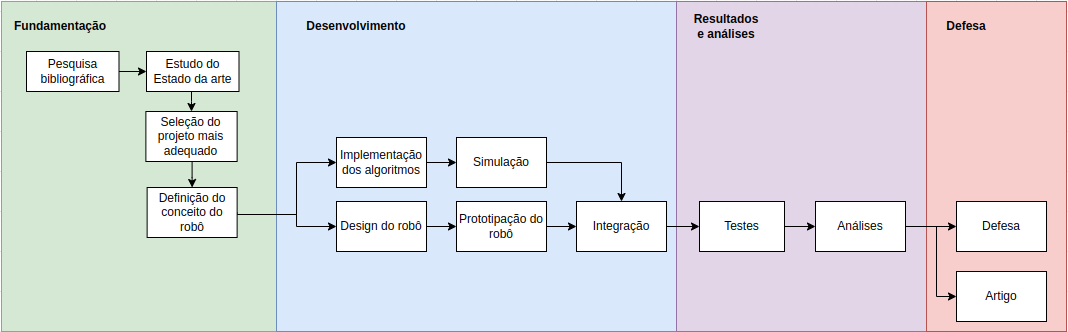
\includegraphics[width=1.0\textwidth]{metodologia.png}
        %\caption{.}
    \end{figure}
    %*----------- notes
    \note[item]{Notes can help you to remember important information. Turn on the notes option.}
\end{frame}
%-

%*----------- SLIDE -------------------------------------------------------------
\begin{frame}[t]{SOTA}
    Aplicamos o método Bili para buscar artigos de referência para o SOTA.

    O foco da pesquisa foi:
    \begin{itemize}
        \item Robô quadrúpede
        \item Design
        \item Estrutura
        \item Controle
    \end{itemize}


    %*----------- notes
    \note[item]{Notes can help you to remember important information. Turn on the notes option.}
\end{frame}
%-

%*----------- SLIDE -------------------------------------------------------------
\begin{frame}[t]{Requisitos}
    \textbf{Requisitos do "cliente":}
    \begin{itemize}
        \item O robô deverá ser capaz de operar por tempo suficiente para inspecionar um ambiente semelhante a uma sala de aula
        \item O robô deverá ser capaz de se locomover em ambientes irregulares
        \item O robô deverá ser capaz de transpor obstáculos pequenos, similares a um livro
        \item O robô deverá atuar em ambientes indoor e outdoor
        \item O transporte do robô deve ser realizado por uma única pessoa utilizando uma maleta
        \item O robô deverá suportar um payload de 2 kg
    \end{itemize}

    %*----------- notes
    \note[item]{Notes can help you to remember important information. Turn on the notes option.}
\end{frame}
%-

%*----------- SLIDE -------------------------------------------------------------
\begin{frame}[t]{Requisitos}
    \textbf{Requisitos técnicos:}
    \begin{itemize}
        \item O robô deverá possuir uma altura máxima de 500 mm
        \item O robô deverá possuir um comprimento máximo de 500 mm
        \item Deverá ter uma massa de, no máximo, 10 kg +/- 1
        \item As juntas devem ser atuadas por servomotores
        \item A relação de massa entre pernas/corpo deve ser a menor possível
        \item O robô deverá ser capaz de transpor obstáculos de até 5cm
        \item O robô deverá ser capaz de operar por, no mínimo, 20 minutos
    \end{itemize}

    %*----------- notes
    \note[item]{Notes can help you to remember important information. Turn on the notes option.}
\end{frame}
%-

%*----------- SLIDE -------------------------------------------------------------
\begin{frame}[t]{QFD}
    \begin{figure}
        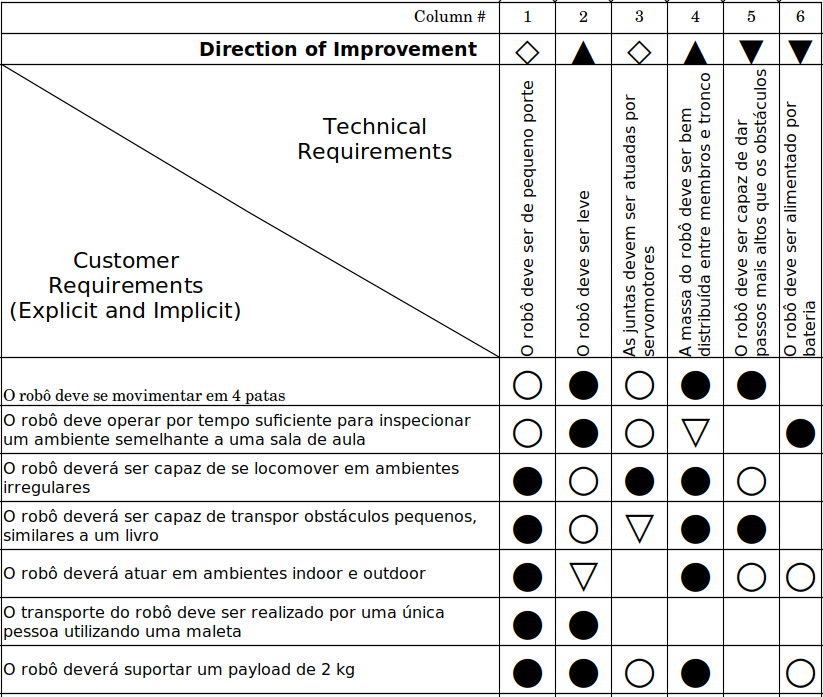
\includegraphics[width=0.5\textwidth]{QFD.png}
        %\caption{.}
    \end{figure}

    %*----------- notes
    \note[item]{Notes can help you to remember important information. Turn on the notes option.}
\end{frame}
%-

%*----------- SLIDE -------------------------------------------------------------
\begin{frame}[t]{QFD}
    \begin{columns}
        \column{.4\textwidth}
        \begin{enumerate}
            \item Deve ser de pequeno porte
            \item Deve ser leve
            \item Juntas atuadas por servomotores
            \item Massa bem distribuída entre corpo e pernas
            \item Deve dar passos mais altos dos que os obstáculos
            \item Deve ser alimentado por bateria
        \end{enumerate}
         \column{.6\textwidth}
        \begin{figure}
            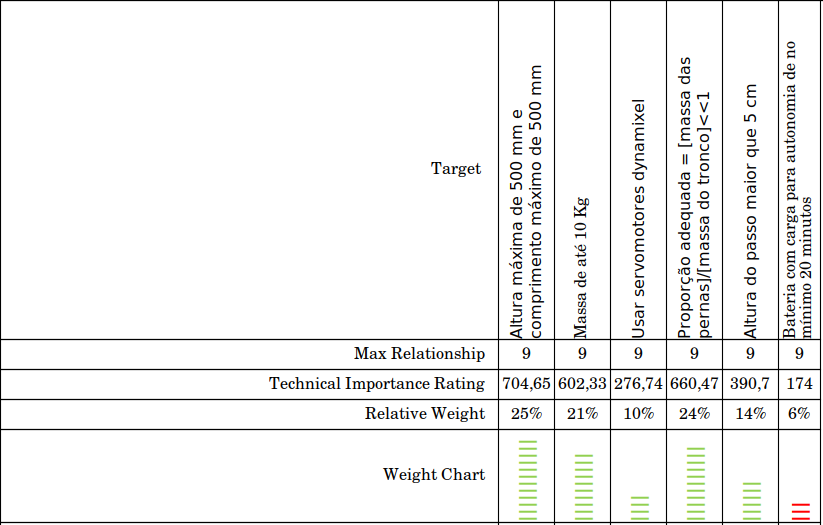
\includegraphics[width=1.0\textwidth]{QFD_2.png}
            %\caption{.}
        \end{figure}
    \end{columns}

    %*----------- notes
    \note[item]{Notes can help you to remember important information. Turn on the notes option.}
\end{frame}
%-
%*----------- SLIDE -------------------------------------------------------------
\begin{frame}[t]{Benchmarking}
 A equipe realizou uma análise entre quatro projetos existentes que estivessem mais próximos do escopo do nosso protótipo.
    \begin{figure}
        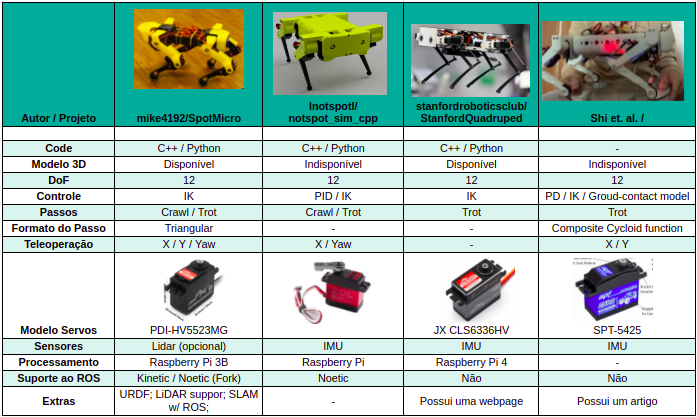
\includegraphics[ width=0.65\textwidth]{benchmarking}
        %\caption{.}
    \end{figure}
    \vspace{1cm}

%*----------- notes
    \note[item]{Notes can help you to remember important information. Turn on the notes option.}
\end{frame}
%-

%*----------- SLIDE -------------------------------------------------------------
\begin{frame}[t]{Arquitetura Geral}
    \begin{figure}
        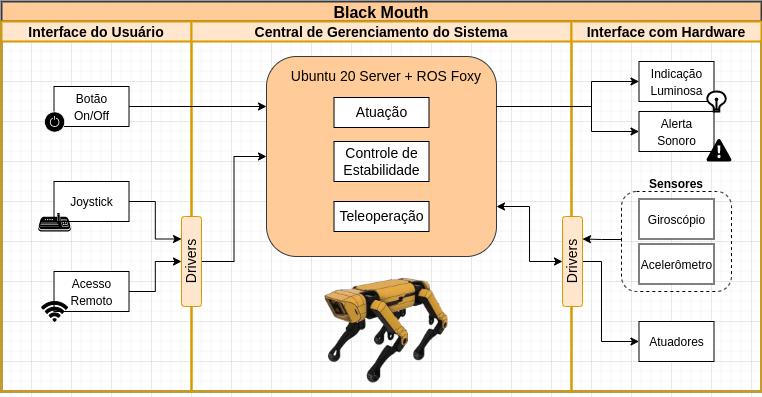
\includegraphics[width=0.85\textwidth]{arquitetura_geral.png}
        %\caption{.}
    \end{figure}
    %*----------- notes
    \note[item]{Notes can help you to remember important information. Turn on the notes option.}
\end{frame}
%-

%*----------- SLIDE -------------------------------------------------------------
\begin{frame}[t]{Project Breakdown Structure}
    \vspace{0.5cm}
    \begin{figure}
        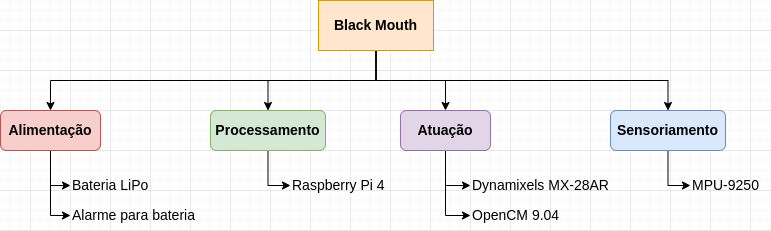
\includegraphics[width=1.0\textwidth]{PBS.png}
        %\caption{.}
    \end{figure}
    %*----------- notes
    \note[item]{Notes can help you to remember important information. Turn on the notes option.}
\end{frame}
%-

%*----------- SLIDE -------------------------------------------------------------
\begin{frame}[t]{Especificação de Funcionalidades}
    \begin{figure}
        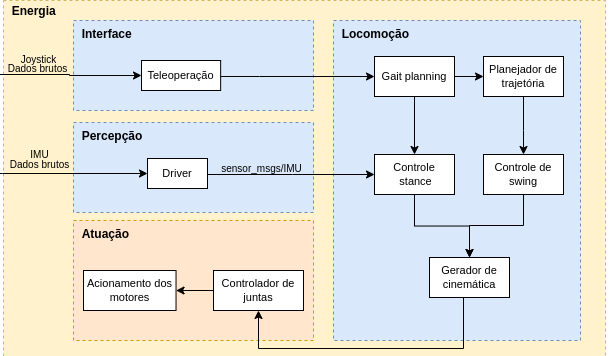
\includegraphics[width=0.78\textwidth]{funcionalidades.png}
        %\caption{.}
    \end{figure}
    %*----------- notes
    \note[item]{Notes can help you to remember important information. Turn on the notes option.}
\end{frame}
%-

%*----------- SLIDE -------------------------------------------------------------
\begin{frame}[t]{Próximas Etapas}
    \begin{columns}
        \begin{column}{0.25\textwidth}
            \begin{figure}
                
\includegraphics[width=1.0\textwidth]{next_steps.png}
                %\caption{.}
            \end{figure}            
        \end{column}
        \begin{column}{0.75\textwidth}
            \begin{itemize}
                \item \textbf{Fundamentação}
                \begin{itemize}
                    \item Finalizar escrita da Introdução
                    \item Finalizar escrita da Metodologia
                    \item Finalizar escrita da Fundamentação Teórica
                    \item Definir do Método de Controle a ser utilizado     
                \end{itemize}
                \item \textbf{Desenvolvimento}
                \begin{itemize}
                    \item Elaborar do CAD mecânico
                    \item Realizar projeto Elétrico-Eletrônico
                \end{itemize}
            \end{itemize}            
        \end{column}
    \end{columns}

    %*----------- notes
    \note[item]{Notes can help you to remember important information. Turn on the notes option.}
\end{frame}
%-

%\input{Sections/04-results}
%\input{Sections/05-references}
%-
%*----------- SLIDE-BACKUP ------------------------------------------------------
% \backupbegin
% %
% \begin{frame}{Backup}
%     Test
% %*----------- notes-------------------------------
% \note{Notes can help you to remember important information. Turn on the notes option.}
% \end{frame}
% %-
% \backupend
% %-
%*----------- QUESTIONS ---------------------------------------------------------
\begin{frame}[c,plain]
    \lastpage{
        \begin{center}
            {\usebeamerfont{title} Questions?}\\[3ex]
            %\hspace{1.5cm} 
            marco.a.reis@google.com
        \end{center}
    }

    %*----------- notes---------------------------------
    \note[item]{Notes can help you to remember important information. Turn on the notes option.}
\end{frame}
%*-------------------------------------------------------------------------------
\end{document}